% ----------------------------------
% Cap Analisis
% ----------------------------------
\chapter{Análisis} % (fold)
	\label{cha:analisis}

	Durante el análisis, se analizan los requisitos que se describieron en la captura de requisitos, refinándolos y estructurándolos. El objetivo de hacerlo es conseguir una comprensión más precisa de los requisitos y una descripción de los mimos que sea fácil de mantener y que ayude a estructurar el sistema entero ---incluyendo su arquitectura.

	El lenguaje que se utiliza en el análisis se basa en un modelo de objetivos conceptual, llamado {\it modelo de análisis}. El modelo de análisis ayuda a refinar los requisitos y a razonar sobre los aspectos internos del sistema, incluidos sus recursos compartidos internos. De hecho, un recurso interno puede representarse como un objeto en el modelo de análisis. Además, el modelo de análisis ofrece un mayor poder expresivo y una mayor formalización, como por ejemplo, la que proporcionan los diagramas de interacción que se utilizan para describir los aspectos dinámicos del sistema.
	
	El modelo de análisis también nos ayuda a estructurar los requisitos como se ha explicado anteriormente y nos proporciona una estructura centrada en el mantenimiento, en aspectos tales como la flexibilidad ante los cambios y la reutilización. Esta estructura no sólo es útil para el mantenimiento de los requisitos como tales, sino que también se utiliza como entrada en las actividades de diseño e implementación. Se trata de preservar esta estructura a medida que se da forma al sistema. Por tanto, el modelo puede considerarse como una primera aproximación al modelo de diseño, aunque es un modelo por sí mismo. Mediante la conservación de la estructura del modelo de análisis durante el diseño, se obtiene un sistema que debería ser también mantenible como un todo: será flexible a los cambios en los requisitos, e incluirá elementos que podrán ser reutilizados cuando se construyan sistemas parecidos.
	
	Sin embargo, es importante hacer notar aquí que el modelo de análisis hace abstracciones, evitando resolver algunos problemas y tratar requisitos que pensamos que es mejor posponer al diseño y a la implementación. Debido a esto, no siempre se puede conservar la estructura proporcionada por el análisis, sino que se debe negociar y comprometer durante el diseño y la implementación. La razón por la cual esta <<conservación de la estructura>> no siempre tiene lugar en la práctica es sencillamente que el diseño debe considerar la plataforma de implementación: lenguaje de programación, sistemas operativos, entornos de trabajo, sistemas heredados y demás.
	
	\newpage
	
	\section{Diagramas de colaboración} % (fold)
		\label{sec:diagramas_de_colaboracion}
	
		Los diagramas de interacción son diagramas que describen cómo grupos de objetos colaboran para conseguir algún fin. Estos diagramas muestran objetos, así como los mensajes que se pasan entre ellos dentro del caso de uso, es decir, capturan el comportamiento de los casos de uso.
		
		Hay dos tipos de diagrama de interacción, ambos basados en la misma información, pero cada uno enfatizando un aspecto particular: Diagramas de Secuencia y {\bf Diagramas de Colaboración}.
		
		Un diagrama de colaboración, se puede decir que es una forma alternativa al diagrama de secuencias a la hora de mostrar un escenario. {\bf Este tipo de diagrama muestra las interacciones que ocurren entre los objetos que participan en una situación determinada.}
		
		En los diagramas de colaboración, se muestran las interacciones entre objetos creando enlaces entre ellos y añadiendo mensajes a esos enlaces. El nombre de un mensaje debería denotar el propósito del objeto invocante en la interacción con el objeto invocado.
		
		En este documento se detallan las principales colaboraciones relacionadas con los principales casos de uso descritos en el proyecto. Por tanto, se detallarán los diagramas de colaboración que hacen referencia a la {\it gestión de acceso, gestión del perfil, gestión de nadadores, gestión de los entrenamientos, gestión de competiciones, gestión test y diario de incidencia.}
		
		\subsection{Colaboraciones para la gestión del acceso} % (fold)
			\label{sub:colaboraciones_para_la_gestion_del_acceso}
		
		La primera de las colaboraciones es la referente al registro de entrenadores en el sistema ({\it véase} Figura \ref{fig:col_registrarse_entrenador}). Dado que es una aplicación distribuida para dar soporte a diferentes entrenadores, éstos tienen que formar parte del sistema  para posteriormente hacer uso de las funcionalidades. 
		
		Una vez que se finaliza el proceso de registro, el entrenador pasa a formar parte del conjunto de actores denominados {\it <<Entrenador Registrado>>}. 
		
			\begin{figure}[H]
			  \centering
			    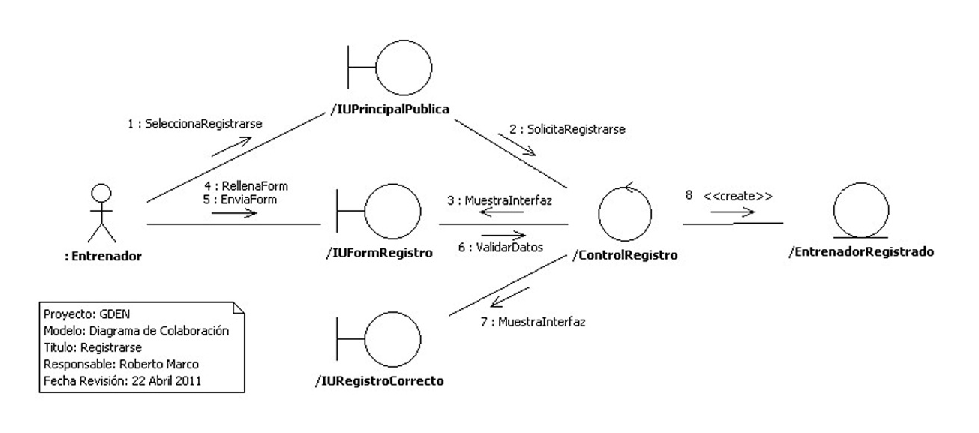
\includegraphics[width=16cm]{./eps/colaboraciones/gestion_acceso/RegistrarseEntrenador.eps}
			  \caption{Diagrama colaboración para registro de entrenador}
			  \label{fig:col_registrarse_entrenador}
			\end{figure}
			
		Seguido del proceso de registro, continúa el de identificación ({\it véase} Figura \ref{fig:col_identificarse_entrenador}) en la aplicación. El entrenador debe acceder al sistema con los datos que insertó en el formulario de registro. En caso de no ser así, fallará la validación. Si no hay ningún error, el controlador de sesión permitirá el inicio de sesión correctamente.
		
			\begin{figure}[H]
			  \centering
			    \includegraphics[width=16cm]{./eps/colaboraciones/gestion_acceso/IdentificarseEntrenador.eps}
			  \caption{Diagrama colaboración para identificación de entrenador}
			  \label{fig:col_identificarse_entrenador}
			\end{figure}
		
		% subsection colaboraciones_para_la_gestión_del_acceso (end)
	
		\subsection{Colaboraciones para la gestión del perfil} % (fold)
			\label{sub:colaboraciones_para_la_gestion_del_perfil}
			
		En la figura \ref{fig:col_cerrar_sesion_entrenador} se muestra el proceso para la finalización de una sesión previamente iniciada.
		
			\begin{figure}[H]
			  \centering
			    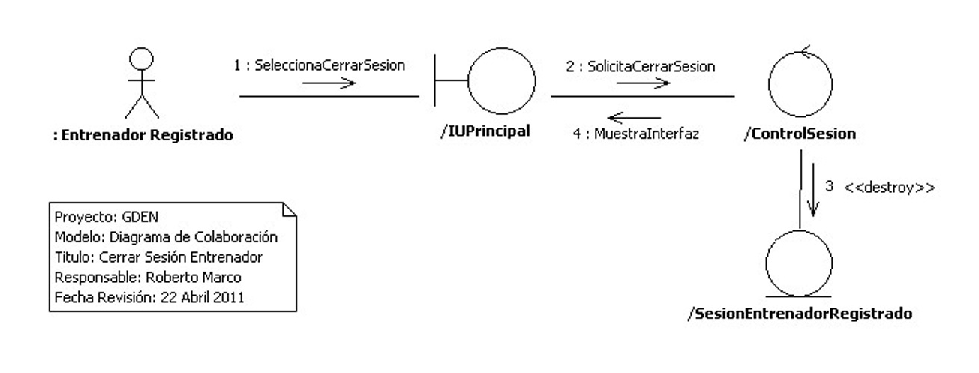
\includegraphics[width=16cm]{./eps/colaboraciones/gestion_perfil/CerrarSesionEntrenador.eps}
			  \caption{Diagrama colaboración para cerrar la sesión de entrenador}
			  \label{fig:col_cerrar_sesion_entrenador}
			\end{figure}
		
		Tras el registro e identificación, cada entrenador es poseedor de un perfil asociado. En él se almacenan los datos personales y de configuración de la sesión. Dada la naturaleza cambiante de la información, el entrenador puede modificar su perfil para actualizar sus datos ({\it véase} Figura \ref{fig:col_modificar_perfil} y \ref{fig:col_cambiar_contrasena}).
			
			\begin{figure}[H]
			  \centering
			    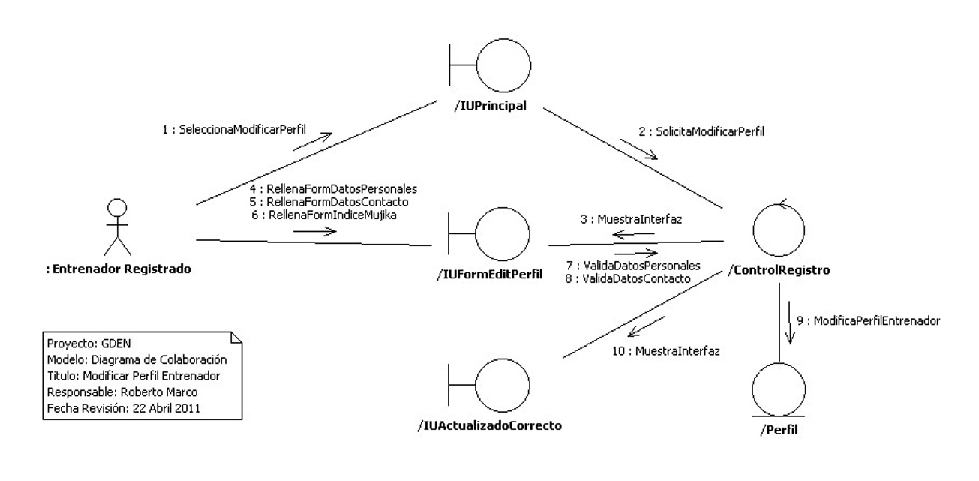
\includegraphics[width=16cm]{./eps/colaboraciones/gestion_perfil/ModificarPerfilEntrenador.eps}
			  \caption{Diagrama colaboración para modificar perfil del entrenador}
			  \label{fig:col_modificar_perfil}
			\end{figure}
			
			\begin{figure}[H]
			  \centering
			    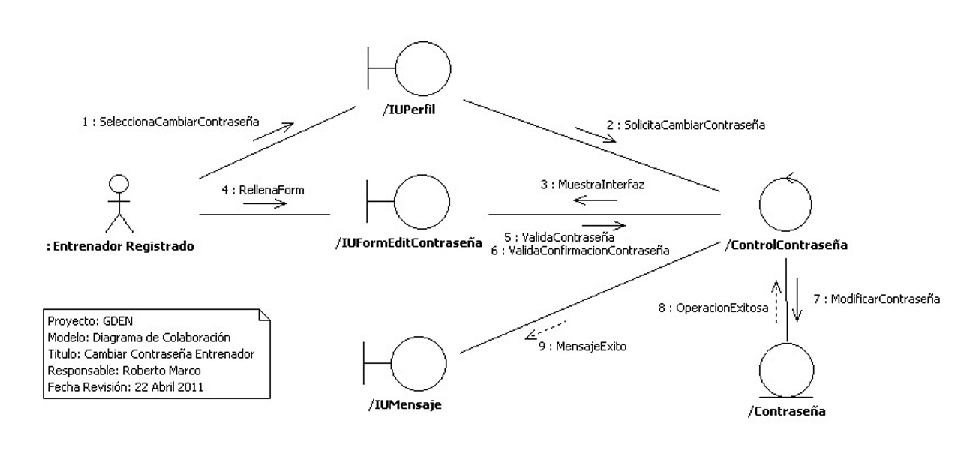
\includegraphics[width=16cm]{./eps/colaboraciones/gestion_perfil/CambiarContrasenaEntrenador.eps}
			  \caption{Diagrama colaboración para cambiar la contraseña del entrenador}
			  \label{fig:col_cambiar_contrasena}
			\end{figure}
		
		% subsection colaboraciones_para_la_gestión_del_perfil (end)
	
		\subsection{Colaboraciones para la gestión de nadadores} % (fold)
			\label{sub:colaboraciones_para_la_gestion_de_nadadores}
		
		La primera de las funcionalidades que se analizará será la de gestión de nadadores pertenecientes a un entrenador registrado. Se selecciona la opción de {\it añadir un nuevo nadador} y se rellenan los datos del formulario mostrado. En caso de éxito, se creará la entidad {\it nadador}.
		
			\begin{figure}[H]
			  \centering
			    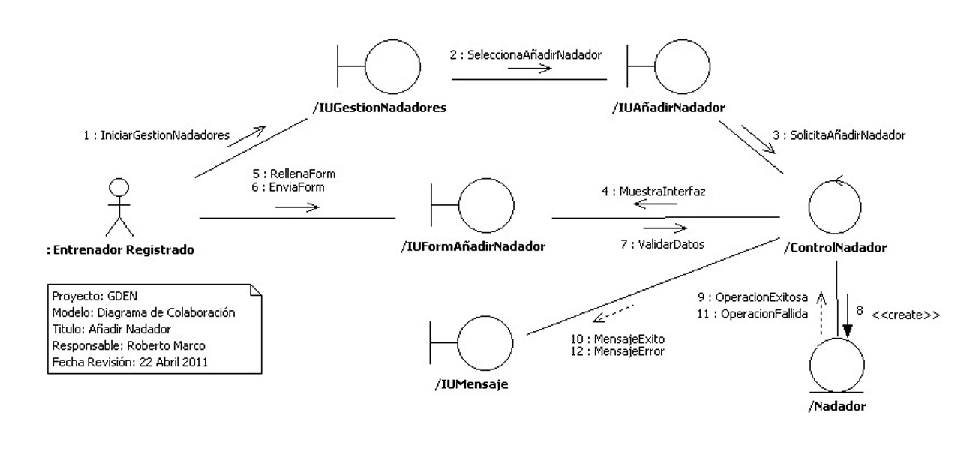
\includegraphics[width=16cm]{./eps/colaboraciones/gestion_nadadores/AnadirNadador.eps}
			  \caption{Diagrama colaboración para añadir nadador}
			  \label{fig:col_anadir_nadador}
			\end{figure}
		
		A medida que se van añadiendo nadadores al sistema, un entrenador está en disposición de ver un listado con los mismos ({\it véase} Figura \ref{fig:col_ver_lista_nadadores}). En la fase de diseño se puede determinar la forma en que se muestra el listado y la ordenación del mismo. De momento, el análisis es una fase más abstracta que no especifica más allá del cómo puede ser el proceso.
			
			\begin{figure}[H]
			  \centering
			    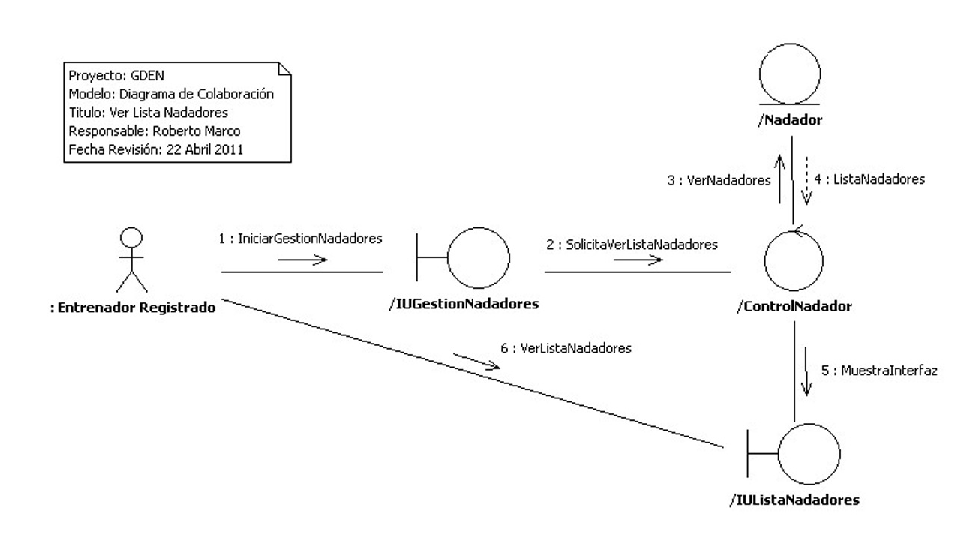
\includegraphics[width=16cm]{./eps/colaboraciones/gestion_nadadores/VerListaNadadores.eps}
			  \caption{Diagrama colaboración para ver lista nadadores}
			  \label{fig:col_ver_lista_nadadores}
			\end{figure}
			
		\newpage
			
			\begin{figure}[H]
			  \centering
			    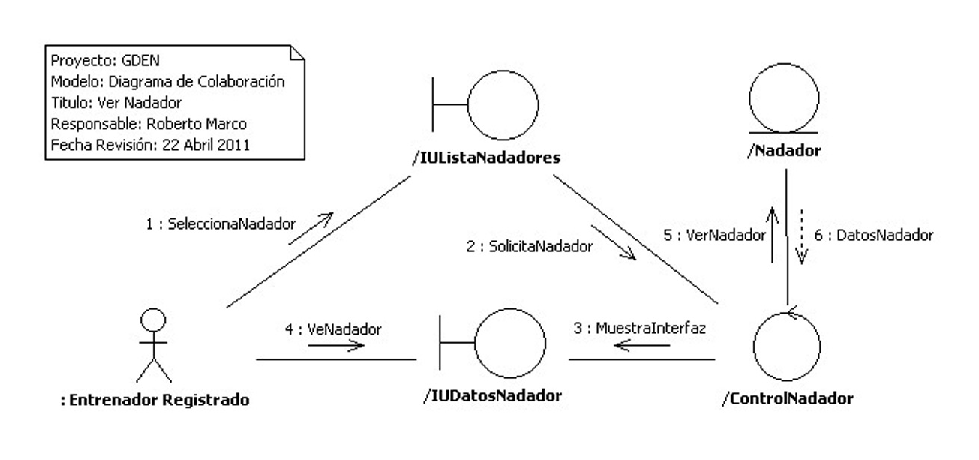
\includegraphics[width=16cm]{./eps/colaboraciones/gestion_nadadores/VerNadador.eps}
			  \caption{Diagrama colaboración para ver nadador}
			  \label{fig:col_ver_nadador}
			\end{figure}
			
		En la figura \ref{fig:col_ver_nadador} se muestra la colaboración para {\it ver un nadador}. El entrenador registrado solicita ver la ficha de un nadador determinado de la lista de nadadores totales. Esto es gestionado por el controlador, mostrando una interfaz con los datos pertinentes. A pesar de que no se refleje en el diagrama, los nadadores tienen resultados de competiciones y test asociados, por lo que se podría hacer una extensión del mismo accediendo a las entidades correspondientes.
		
			\begin{figure}[H]
			  \centering
			    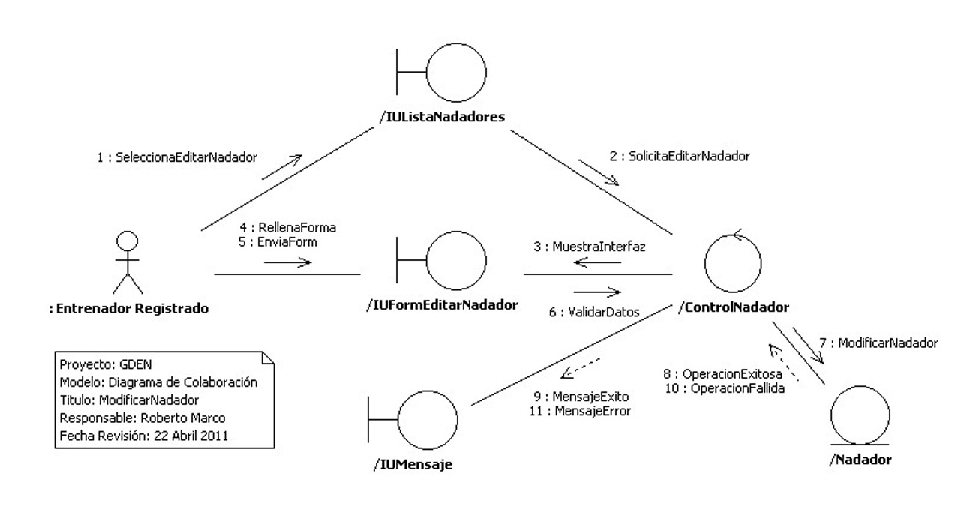
\includegraphics[width=16cm]{./eps/colaboraciones/gestion_nadadores/ModificarNadador.eps}
			  \caption{Diagrama colaboración para modificar nadador}
			  \label{fig:col_modificar_nadador}
			\end{figure}
			
			\begin{figure}[H]
			  \centering
			    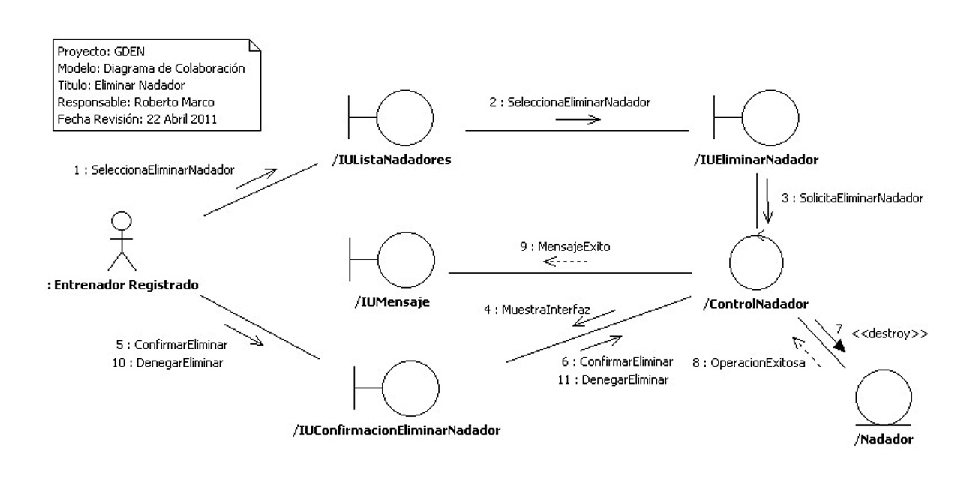
\includegraphics[width=16cm]{./eps/colaboraciones/gestion_nadadores/EliminarNadador.eps}
			  \caption{Diagrama colaboración para eliminar nadador}
			  \label{fig:col_eliminar_nadador}
			\end{figure}
		
		Tanto para la modificación como eliminación de un nadador ({\it véase} Figuras \ref{fig:col_modificar_nadador} y \ref{fig:col_eliminar_nadador}) el proceso es muy similar. La salvedad es que uno muestra un formulario editable para poder actualizar la información y el otro elimina un registro concreto perteneciente al entrenador registrado. Aunque en el diagrama no aparezca, en fases posteriores la colaboración tiene que ser extendida para poder eliminar los registros de resultados de competiciones y test asociados a un nadador.
		
		Para el resto de colaboraciones únicamente se mostrarán los diagramas debido a que los procesos son muy parecidos.
			
		% subsection colaboraciones_para_la_gestión_de_nadadores (end)
		
		\subsection{Colaboraciones para la gestión de entrenamientos} % (fold)
			\label{sub:colaboraciones_para_la_gestion_de_entrenamientos}
		
			\begin{figure}[H]
			  \centering
			    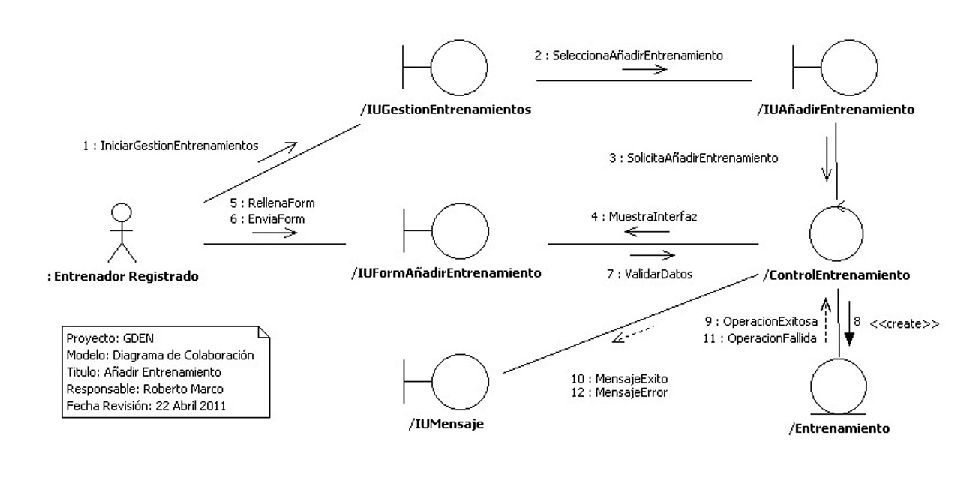
\includegraphics[width=16cm]{./eps/colaboraciones/gestion_entrenamiento/AnadirEntrenamiento.eps}
			  \caption{Diagrama colaboración para añadir entrenamiento}
			  \label{fig:col_anadir_entrenamiento}
			\end{figure}
			
			\begin{figure}[H]
			  \centering
			    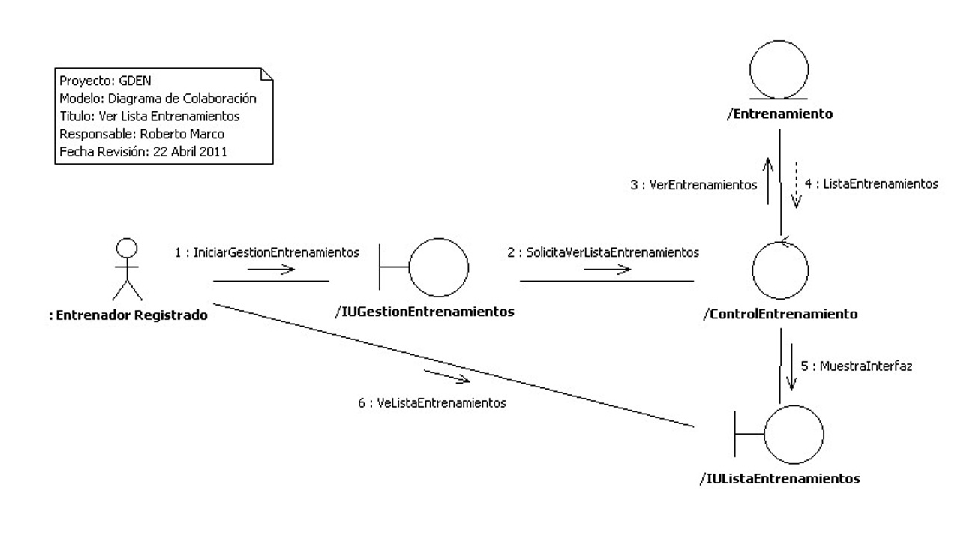
\includegraphics[width=16cm]{./eps/colaboraciones/gestion_entrenamiento/VerListaEntrenamientos.eps}
			  \caption{Diagrama colaboración para ver lista de entrenamientos}
			  \label{fig:col_ver_lista_entrenamientos}
			\end{figure}
			
			\begin{figure}[H]
			  \centering
			    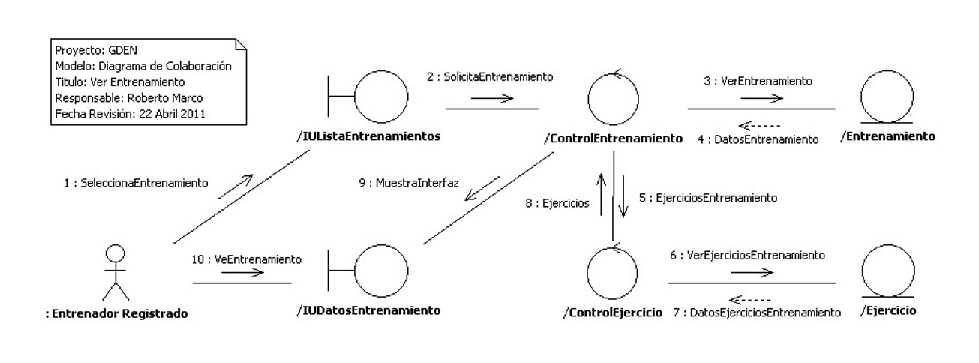
\includegraphics[width=16cm]{./eps/colaboraciones/gestion_entrenamiento/VerEntrenamiento.eps}
			  \caption{Diagrama colaboración para ver entrenamiento}
			  \label{fig:col_ver_entrenamiento}
			\end{figure}
			
			\begin{figure}[H]
			  \centering
			    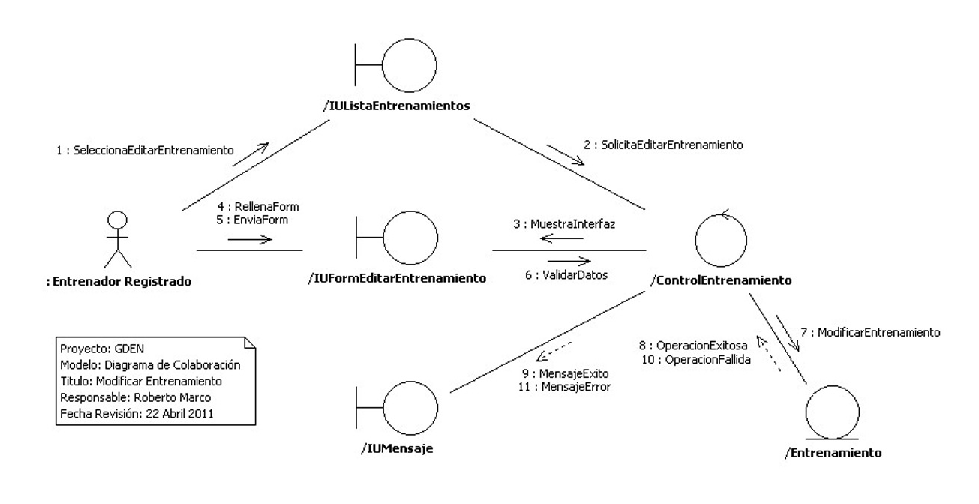
\includegraphics[width=16cm]{./eps/colaboraciones/gestion_entrenamiento/ModificarEntrenamiento.eps}
			  \caption{Diagrama colaboración para modificar entrenamiento}
			  \label{fig:col_modificar_entrenamiento}
			\end{figure}
			
			\begin{figure}[H]
			  \centering
			    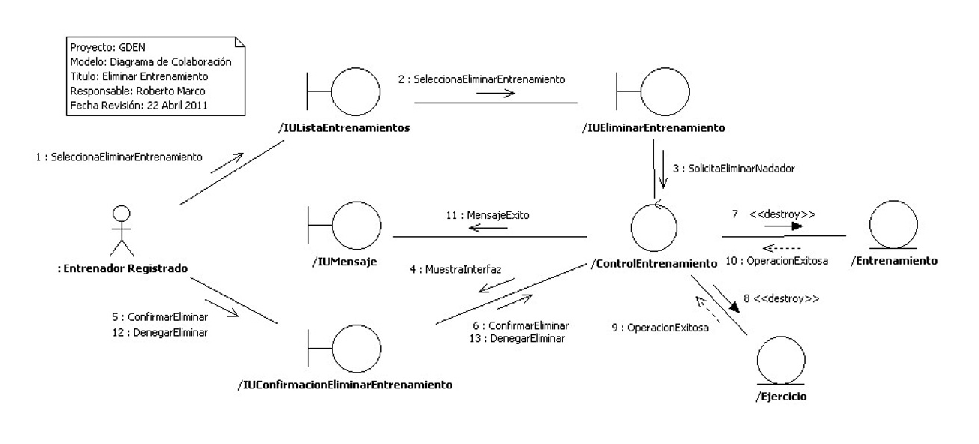
\includegraphics[width=16cm]{./eps/colaboraciones/gestion_entrenamiento/EliminarEntrenamiento.eps}
			  \caption{Diagrama colaboración para eliminar entrenamiento}
			  \label{fig:col_eliminar_entrenamiento}
			\end{figure}
		% subsection colaboraciones_para_la_gestión_de_entrenamientos (end)
	
		\subsection{Colaboraciones para la gestión de competiciones} % (fold)
			\label{sub:colaboraciones_para_la_gestion_de_competiciones}
		
			\begin{figure}[H]
			  \centering
			    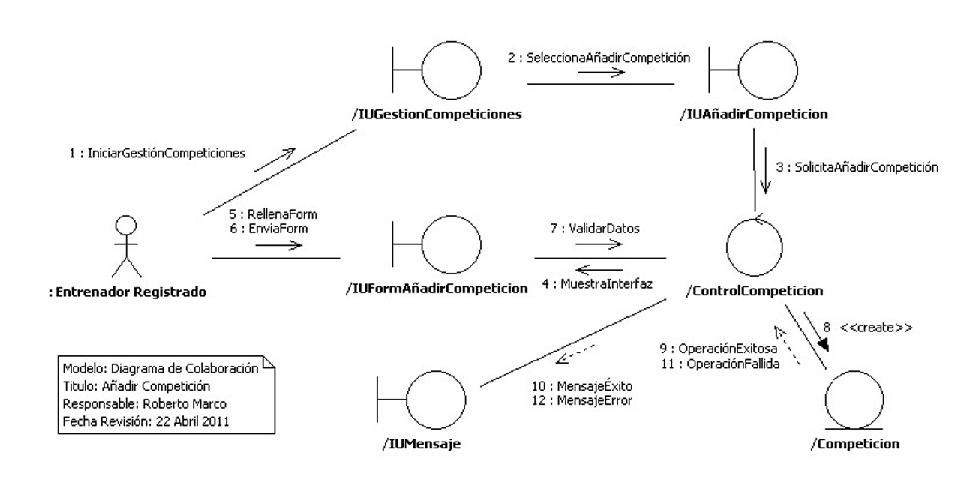
\includegraphics[width=16cm]{./eps/colaboraciones/gestion_competiciones/AnadirCompeticion.eps}
			  \caption{Diagrama colaboración para añadir competición}
			  \label{fig:col_anadir_competicion}
			\end{figure}
			
			\begin{figure}[H]
			  \centering
			    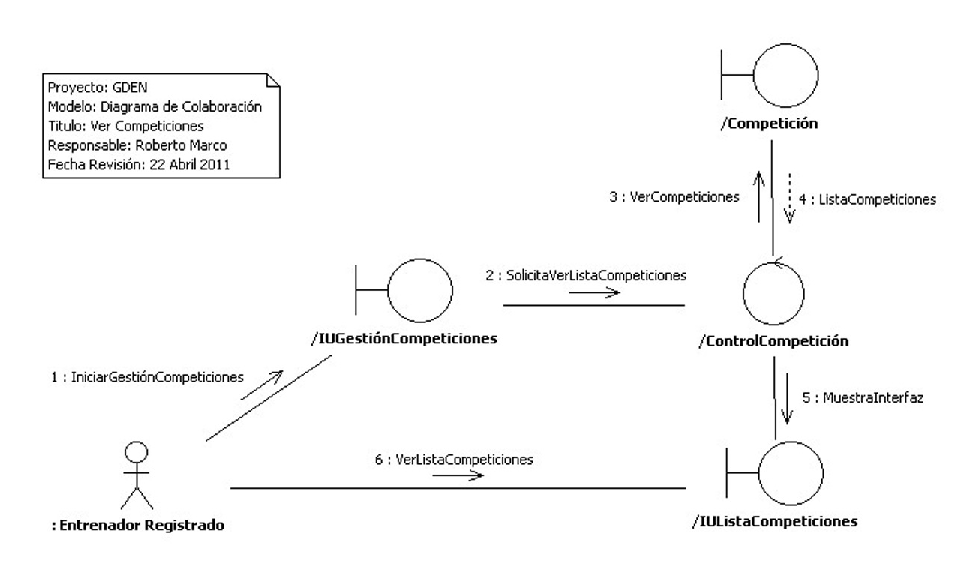
\includegraphics[width=16cm]{./eps/colaboraciones/gestion_competiciones/VerListaCompeticiones.eps}
			  \caption{Diagrama colaboración para ver lista de competiciones}
			  \label{fig:col_ver_lista_competiciones}
			\end{figure}
			
			\begin{figure}[H]
			  \centering
			    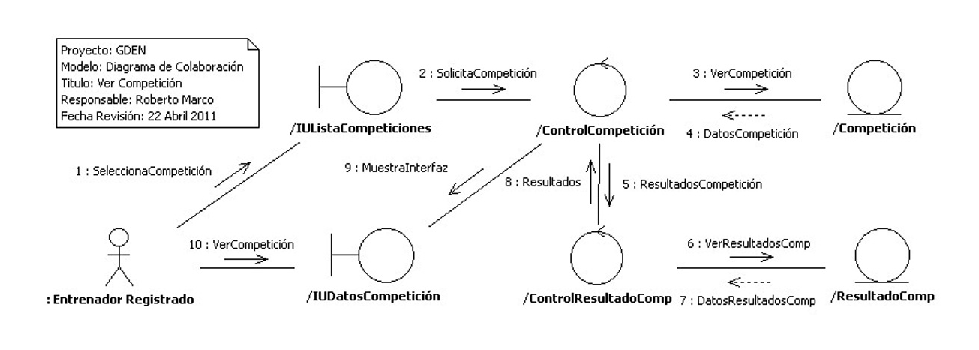
\includegraphics[width=16cm]{./eps/colaboraciones/gestion_competiciones/VerCompeticion.eps}
			  \caption{Diagrama colaboración para ver competición}
			  \label{fig:col_ver_competicion}
			\end{figure}
			
			\begin{figure}[H]
			  \centering
			    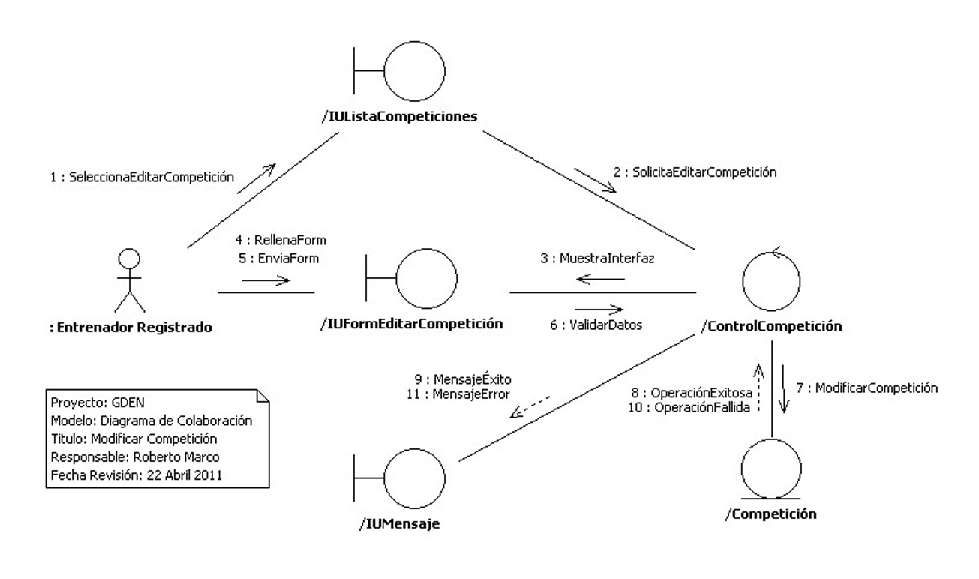
\includegraphics[width=16cm]{./eps/colaboraciones/gestion_competiciones/ModificarCompeticion.eps}
			  \caption{Diagrama colaboración para modificar competición}
			  \label{fig:col_modificar_competicion}
			\end{figure}
			
			\begin{figure}[H]
			  \centering
			    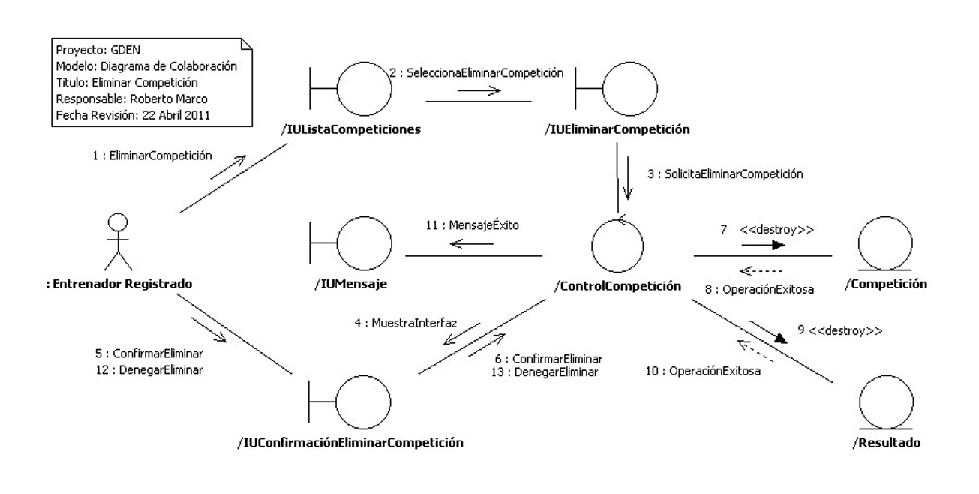
\includegraphics[width=16cm]{./eps/colaboraciones/gestion_competiciones/EliminarCompeticion.eps}
			  \caption{Diagrama colaboración para eliminar competición}
			  \label{fig:col_eliminar_competicion}
			\end{figure}
			
		% subsection colaboraciones_para_la_gestión_de_competiciones (end)
		
		\subsection{Colaboraciones para la gestión de test} % (fold)
			\label{sub:colaboraciones_para_la_gestion_de_test}
			
			\begin{figure}[H]
			  \centering
			    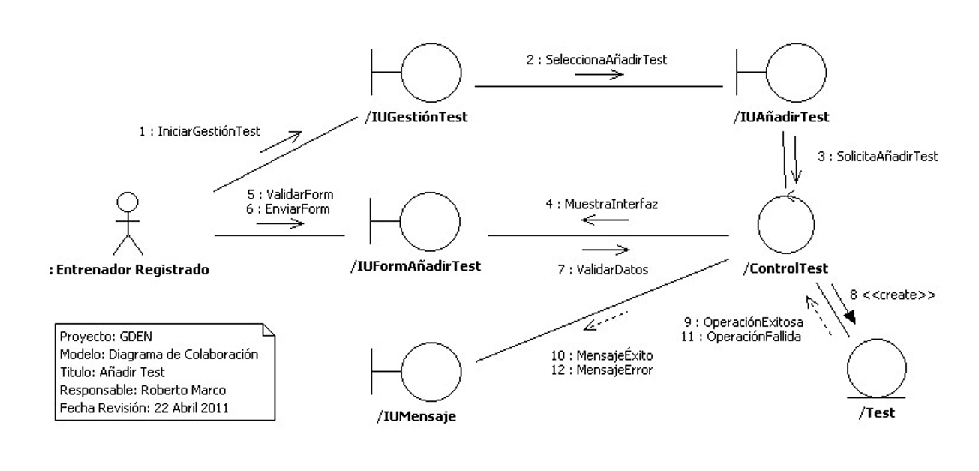
\includegraphics[width=16cm]{./eps/colaboraciones/gestion_test/AnadirTest.eps}
			  \caption{Diagrama colaboración para añadir test}
			  \label{fig:col_anadir_test}
			\end{figure}
			
			\begin{figure}[H]
			  \centering
			    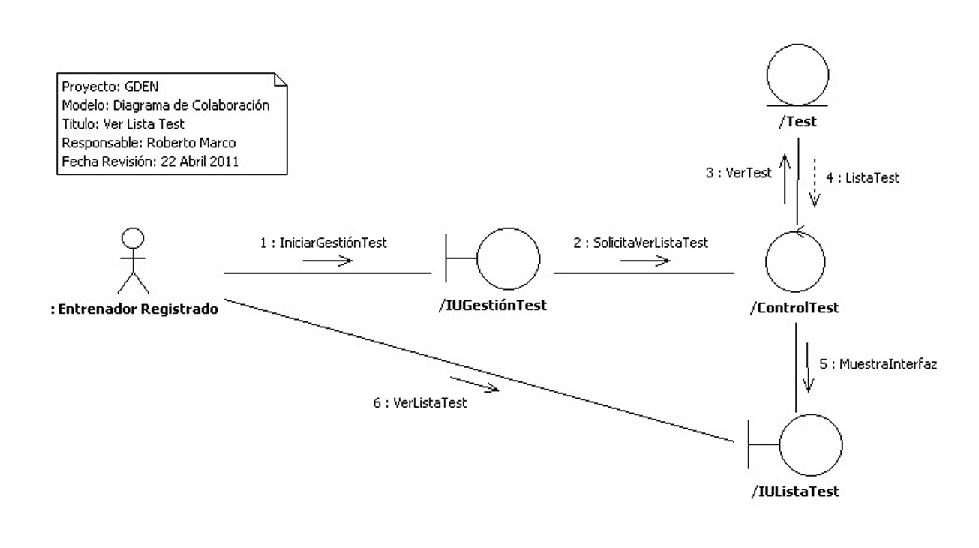
\includegraphics[width=16cm]{./eps/colaboraciones/gestion_test/VerListaTest.eps}
			  \caption{Diagrama colaboración para ver lista test}
			  \label{fig:col_ver_lista_test}
			\end{figure}
			
			\begin{figure}[H]
			  \centering
			    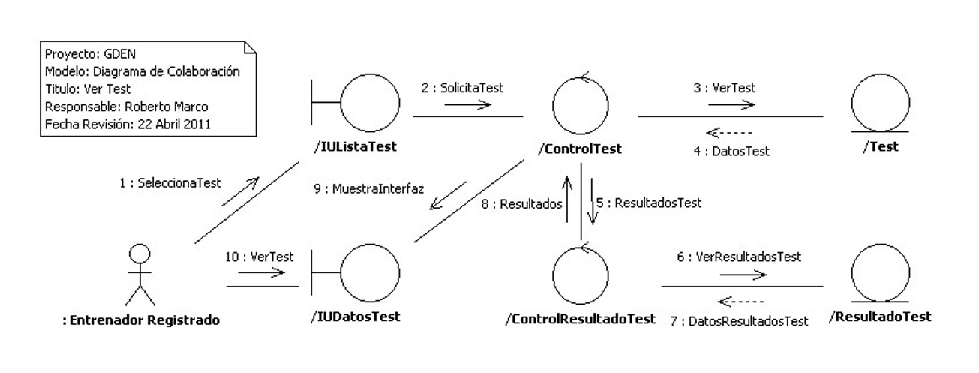
\includegraphics[width=16cm]{./eps/colaboraciones/gestion_test/VerTest.eps}
			  \caption{Diagrama colaboración para ver test}
			  \label{fig:col_ver_test}
			\end{figure}
			
			\begin{figure}[H]
			  \centering
			    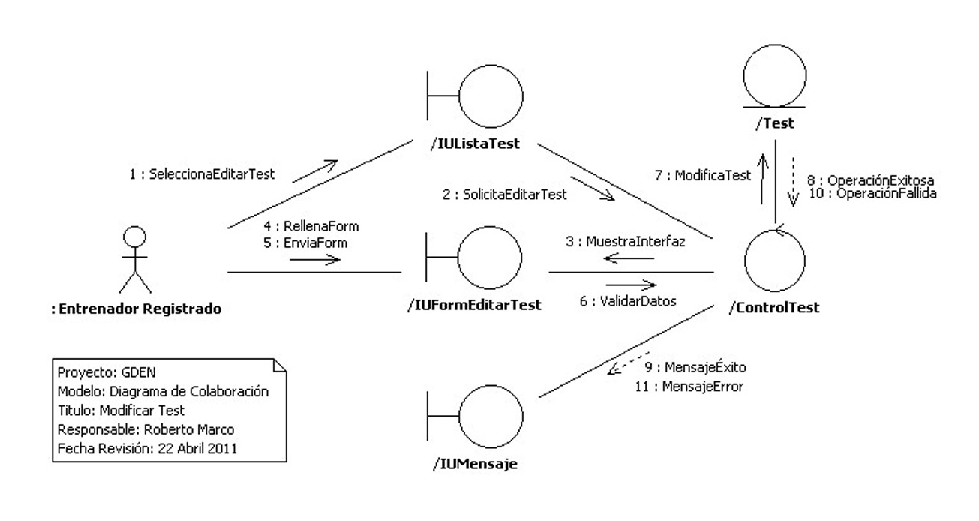
\includegraphics[width=16cm]{./eps/colaboraciones/gestion_test/ModificarTest.eps}
			  \caption{Diagrama colaboración para modificar test}
			  \label{fig:col_modificar_test}
			\end{figure}
			
			\begin{figure}[H]
			  \centering
			    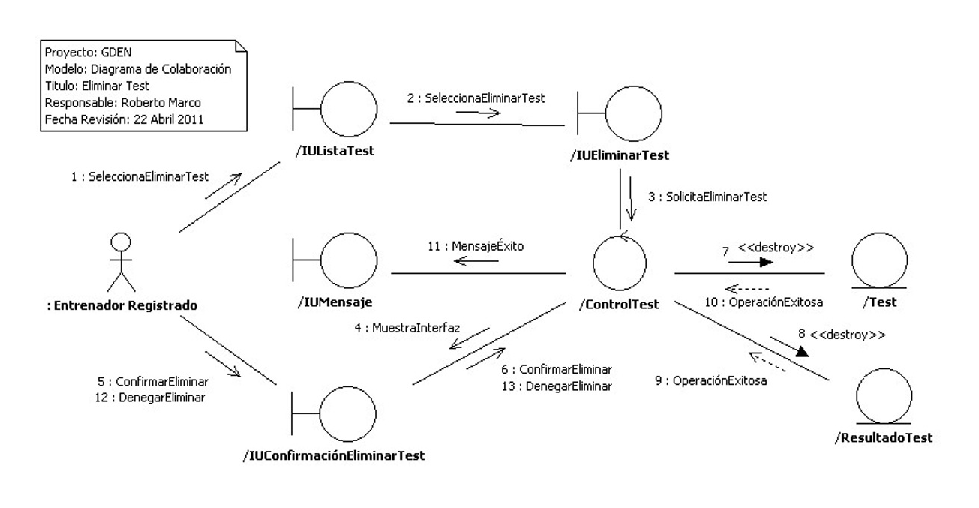
\includegraphics[width=16cm]{./eps/colaboraciones/gestion_test/EliminarTest.eps}
			  \caption{Diagrama colaboración para eliminar test}
			  \label{fig:col_eliminar_test}
			\end{figure}
		
		% subsection colaboraciones_para_la_gestión_de_test (end)
		
		\subsection{Colaboraciones para la gestión del diario de incidencias} % (fold)
			\label{sub:colaboraciones_para_la_gestion_del_diario_de_incidencias}
			
			\begin{figure}[H]
			  \centering
			    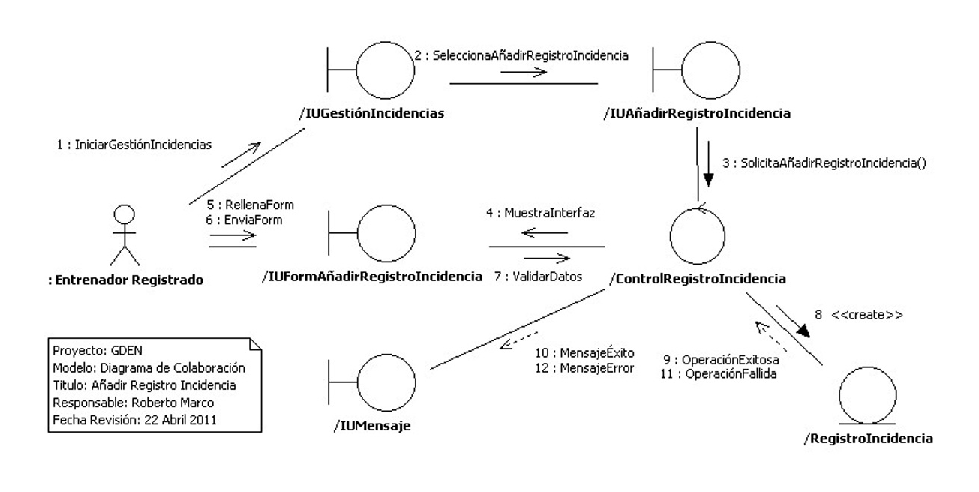
\includegraphics[width=16cm]{./eps/colaboraciones/gestion_diarioincidencia/AnadirRegistroIncidencia.eps}
			  \caption{Diagrama colaboración para añadir incidencia}
			  \label{fig:col_anadir_incidencia}
			\end{figure}
			
			\begin{figure}[H]
			  \centering
			    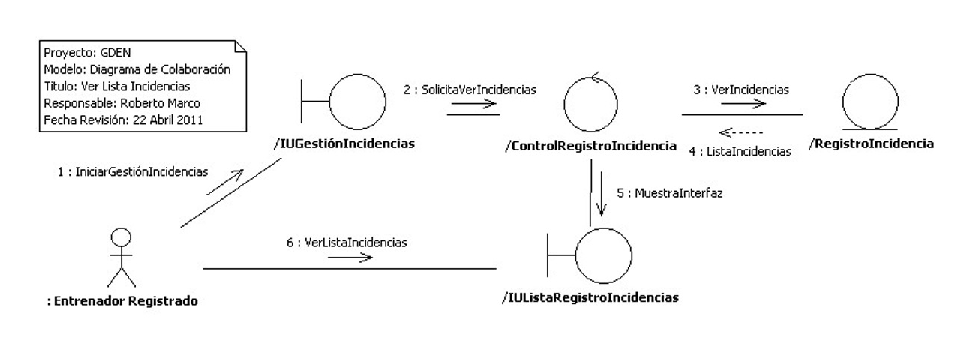
\includegraphics[width=16cm]{./eps/colaboraciones/gestion_diarioincidencia/VerListaRegistroIncidencias.eps}
			  \caption{Diagrama colaboración para ver lista de incidencias}
			  \label{fig:col_ver_lista_incidencias}
			\end{figure}
			
			\begin{figure}[H]
			  \centering
			    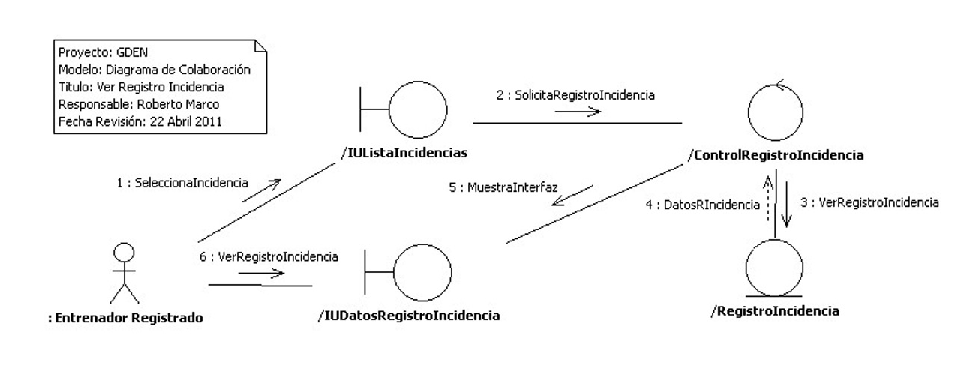
\includegraphics[width=16cm]{./eps/colaboraciones/gestion_diarioincidencia/VerRegistroIncidencia.eps}
			  \caption{Diagrama colaboración para ver incidencia}
			  \label{fig:col_ver_incidencia}
			\end{figure}
			
			\begin{figure}[H]
			  \centering
			    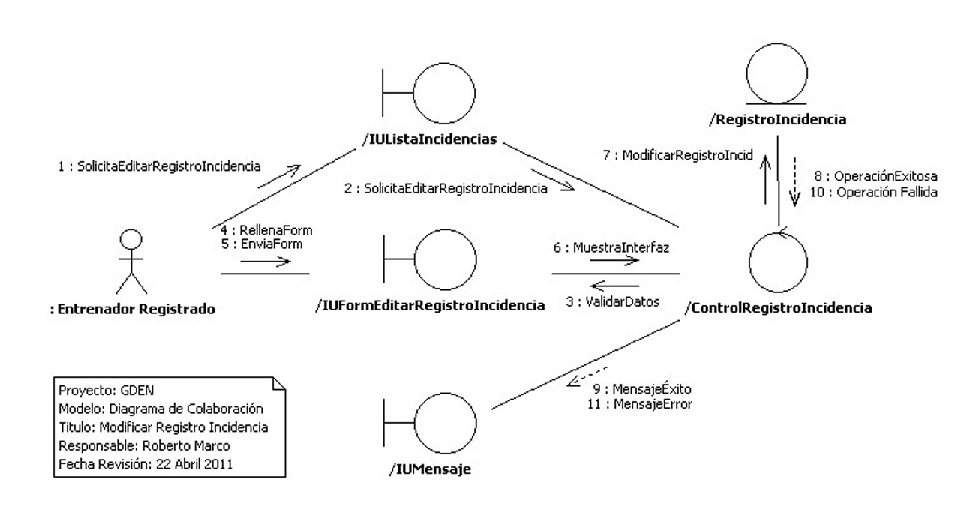
\includegraphics[width=16cm]{./eps/colaboraciones/gestion_diarioincidencia/ModificarRegistroIncidencia.eps}
			  \caption{Diagrama colaboración para modificar incidencia}
			  \label{fig:col_modificar_incidencia}
			\end{figure}
			
			\begin{figure}[H]
			  \centering
			    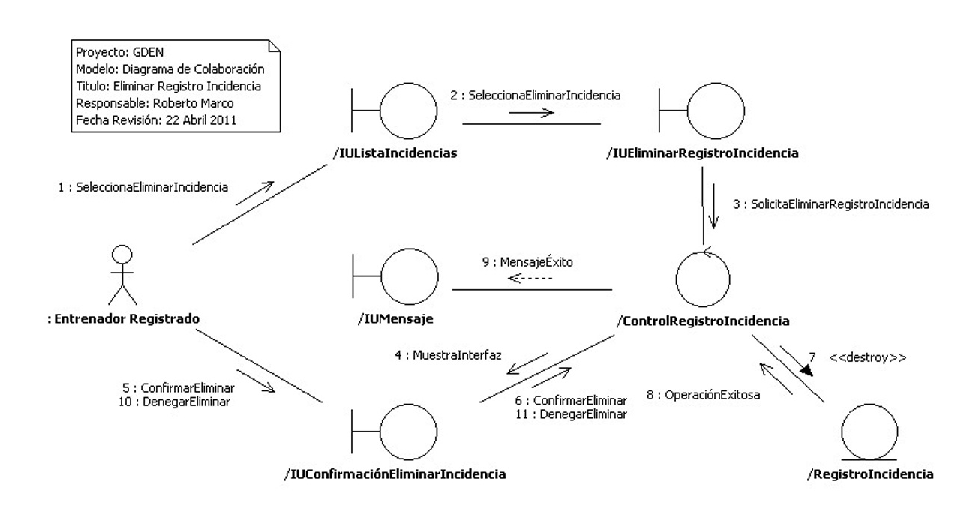
\includegraphics[width=16cm]{./eps/colaboraciones/gestion_diarioincidencia/EliminarRegistroIncidencia.eps}
			  \caption{Diagrama colaboración para eliminar incidencia}
			  \label{fig:col_eliminar_incidencia}
			\end{figure}
		% subsection colaboraciones_para_la_gestión_del_diario_de_incidencias (end)
	% section diagramas_de_colaboración (end)
		
	\section{Diagrama de clases} % (fold)
		\label{sec:diagrama_de_clases}
		
		Los autores Jacobson, Booch y Rumbaugh definen en la guía del proceso unificado de desarrollo de software \cite{PUJac08} una clase de análisis como: {\it <<una abstracción de una o varias clases y/o subsistemas del diseño del sistema>>}. Esta abstracción posee las siguientes características:
		
		\begin{itemize}
			\item Una clase de análisis se centra en el tratamiento de los requisitos funcionales y pospone los no funcionales.
			\item Esto hace que una clase de análisis sea más evidente en el contexto del dominio del problema, a menudo de mayor granularidad que sus contrapartidas de diseño e implementación.
			\item Una clase de análisis raramente define u ofrece un interfaz en términos de operaciones y de sus signaturas. Sin embargo, su comportamiento se define mediante responsabilidades en un nivel más alto y menos formal.
			\item Una clase de análisis define atributos, aunque esos atributos también son de un nivel bastante alto.
			\item Una clase de análisis participa en relaciones, aunque esas relaciones son más conceptuales que sus contrapartidas de diseño e implementación.
			\item Las clases de análisis siempre encajan en uno de tres estereotipos básicos: de interfaz, de control o de entidad.
		\end{itemize}
		
		\subsection{Nadadores} % (fold)
			\label{sub:nadadores}
		
			\begin{figure}[H]
			  \centering
			    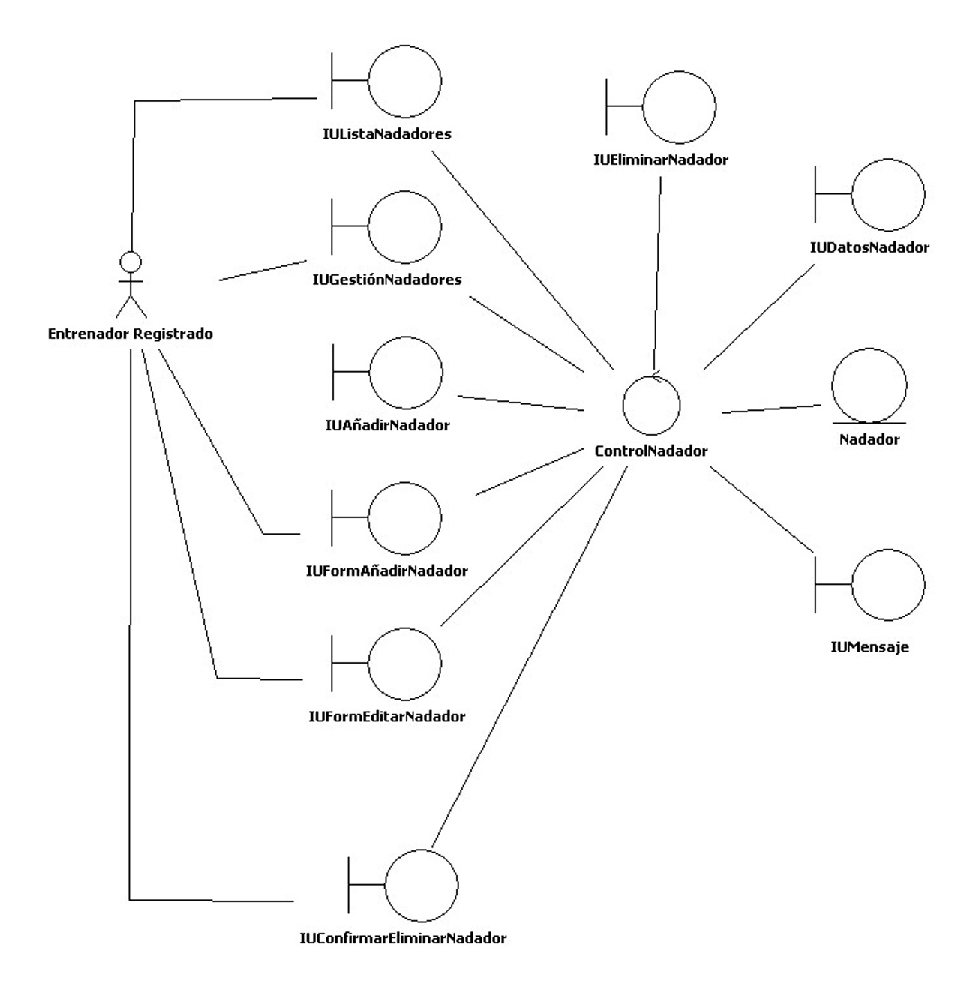
\includegraphics[width=14cm]{./eps/an_diagclases/GestionNadadores.eps}
			  \caption{Diagrama de clases Nadadores}
			  \label{fig:an_diagclases_nadadores}
			\end{figure}
			
		% subsection nadadores (end)
	
		\subsection{Competiciones} % (fold)
			\label{sub:competiciones}
		
			\begin{figure}[H]
			  \centering
			    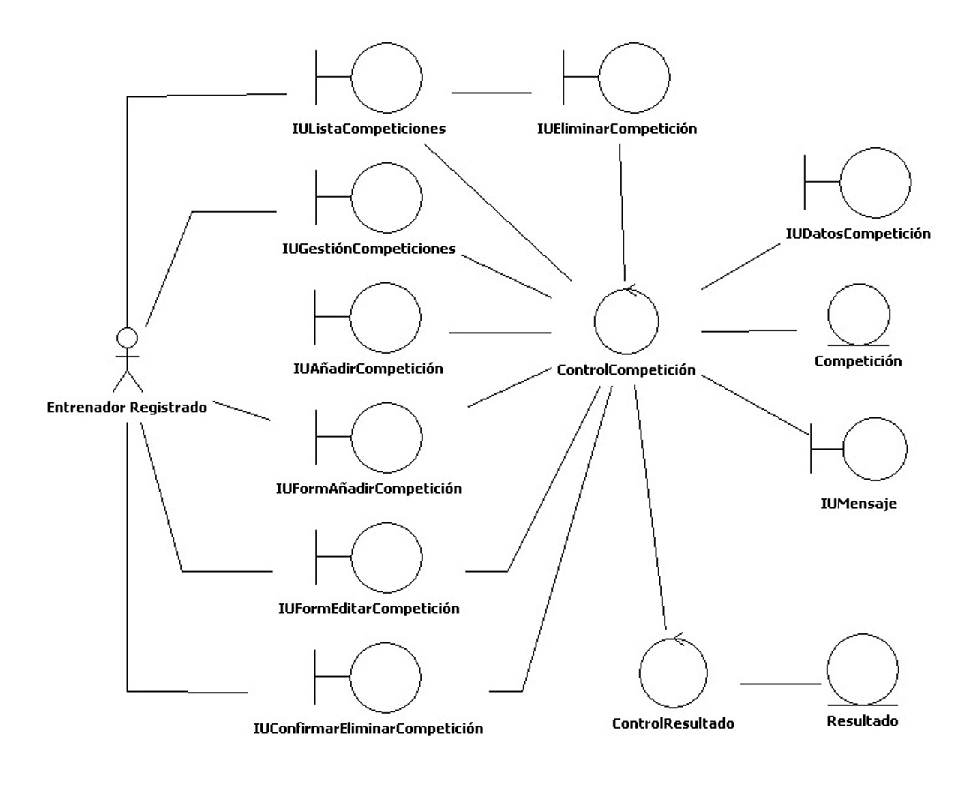
\includegraphics[width=14cm]{./eps/an_diagclases/GestionCompeticiones.eps}
			  \caption{Diagrama de clases Competiciones}
			  \label{fig:an_diagclases_competiciones}
			\end{figure}
		% subsection competiciones (end)
		
		\subsection{Entrenamientos} % (fold)
			\label{sub:entrenamientos}
			
			\begin{figure}[H]
			  \centering
			    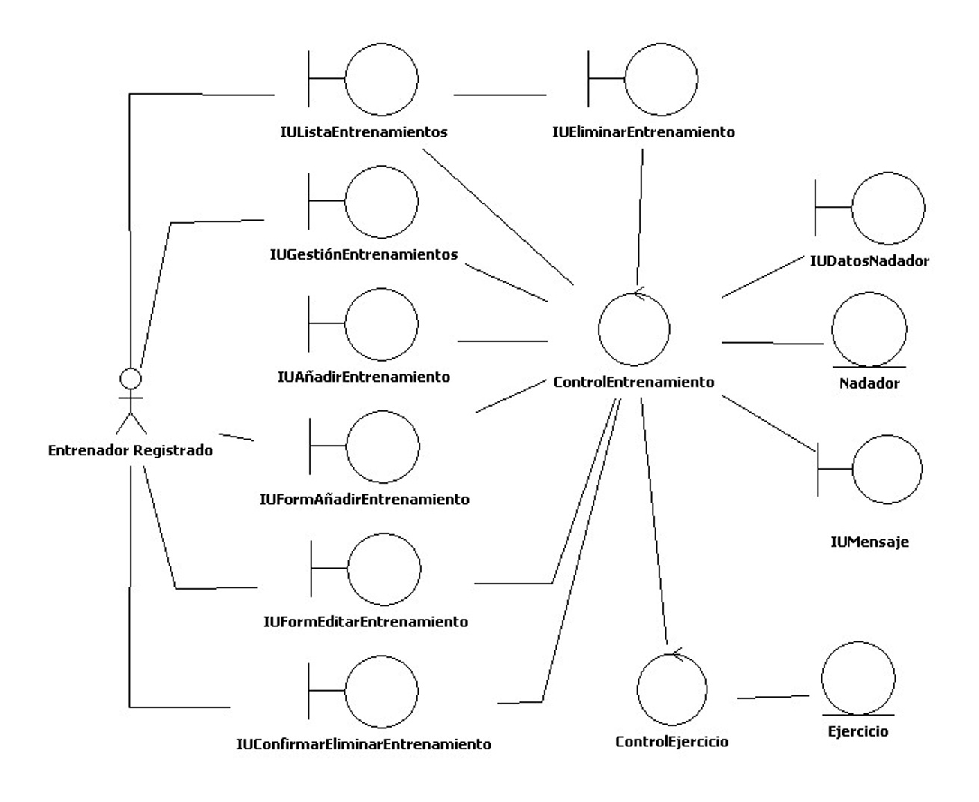
\includegraphics[width=14cm]{./eps/an_diagclases/GestionEntrenamientos.eps}
			  \caption{Diagrama de clases Entrenamientos}
			  \label{fig:an_diagclases_entrenamientos}
			\end{figure}
		% subsection entrenamientos (end)
		
		\subsection{Test} % (fold)
			\label{sub:test}
			
			\begin{figure}[H]
			  \centering
			    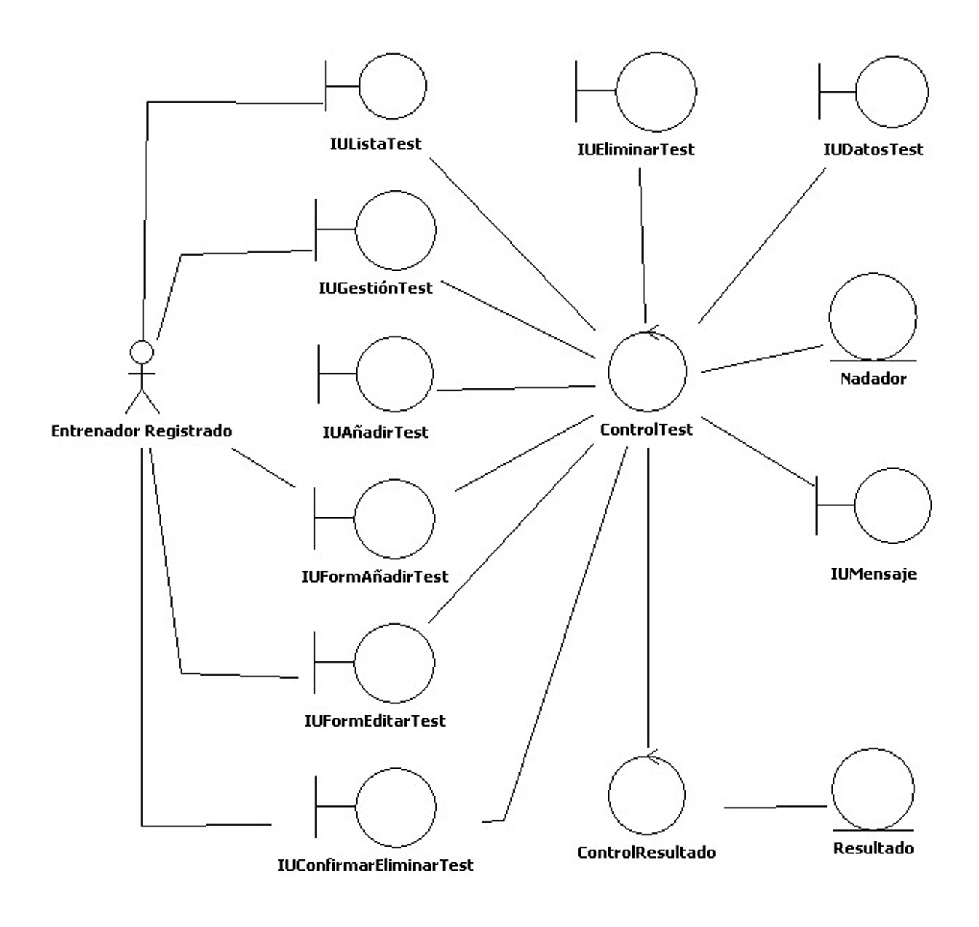
\includegraphics[width=14cm]{./eps/an_diagclases/GestionTest.eps}
			  \caption{Diagrama de clases Test}
			  \label{fig:an_diagclases_test}
			\end{figure}
		% subsection test (end)
		
		\subsection{Diario de Incidencias} % (fold)
			\label{sub:diario_de_incidencias}
			
			\begin{figure}[H]
			  \centering
			    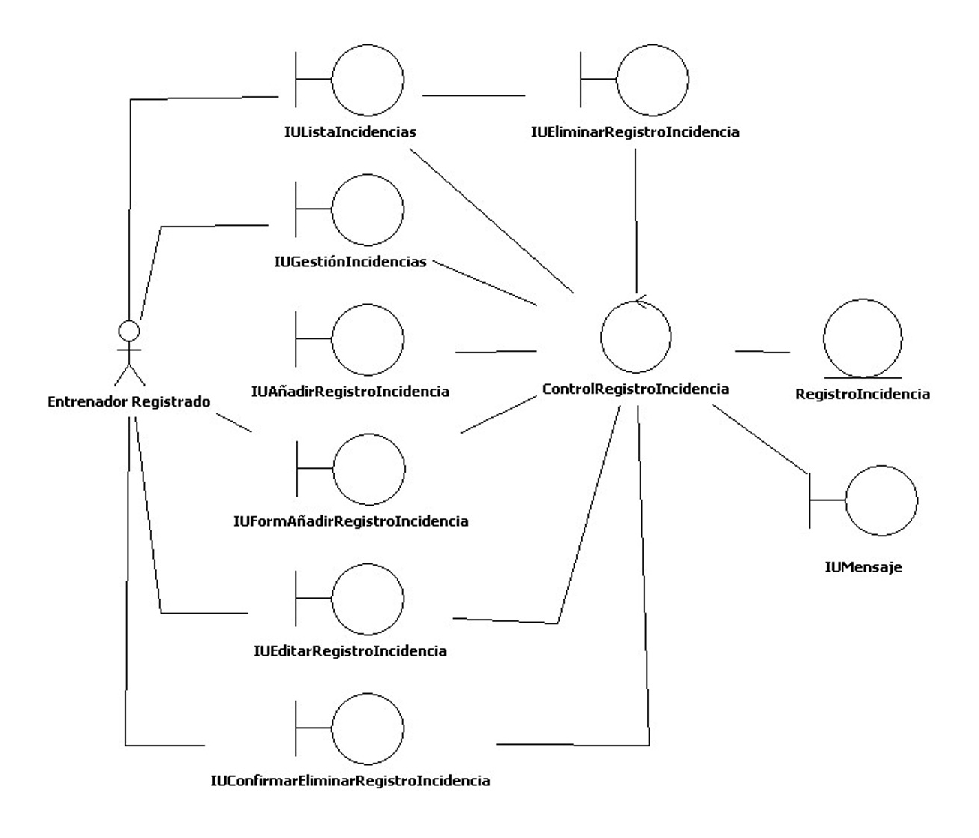
\includegraphics[width=14cm]{./eps/an_diagclases/GestionIncidencias.eps}
			  \caption{Diagrama de clases Incidencias}
			  \label{fig:an_diagclases_incidencias}
			\end{figure}
		% subsection diario_de_incidencias (end)
	% section diagrama_de_clases (end)	
	
	\section{Diagrama de paquetes} % (fold)
		\label{sec:diagrama_de_paquetes_analisis}
		
		Es la metodología del proceso unificado, es el arquitecto de software quien realiza un {\bf análisis de la arquitectura}. El propósito de este análisis es esbozar el modelo de análisis y la arquitectura mediante la identificación de paquetes del análisis, clases del análisis evidentes y requisitos especiales comunes.
		
		Los {\bf paquetes del análisis} proporcionan un medio para organizar el modelo de análisis en piezas más pequeñas y más manejables. Puede, bien identificarse inicialmente como forma de dividir el trabajo de análisis, o bien encontrase a medida que el modelo de análisis evoluciona y <<crece>>, convirtiéndose en una gran estructura que debe descomponerse.
		
		Una identificación inicial de los paquetes del análisis se hace de manera natural basándonos en los requisitos funcionales y en el dominio del problema, es decir, en la aplicación que estamos considerando. Debido a que capturamos los requisitos funcionales en la forma de casos de uso, una forma directa de identificar paquetes del análisis es asignar la mayor parte de un cierto número de casos de uso a un paquete concreto y, posteriormente, realizar la funcionalidad correspondiente dentro de ese paquete. Entre las <<asignaciones>> adecuadas de casos de uso a un paquete en concreto se tienen las siguientes:
		\begin{itemize}
			\item Los casos de uso requeridos para dar soporte a un determinado proceso de negocio.
			\item Los casos de uso requeridos para dar soporte a un determinado actor del sistema.
			\item Los casos de uso que están relacionados mediante relaciones de generalización y de extensión.
		\end{itemize}
		
		La arquitectura del sistema estará dividida en diferentes capas: {\it capa específica, capa genérica, capa middleware o entorno de trabajo y capa del sistema operativo}. En el análisis se dará forma a las dos primeras, lo que ayudará a tener una base para la fase de diseño.
		
		\begin{figure}[H]
		  \centering
		    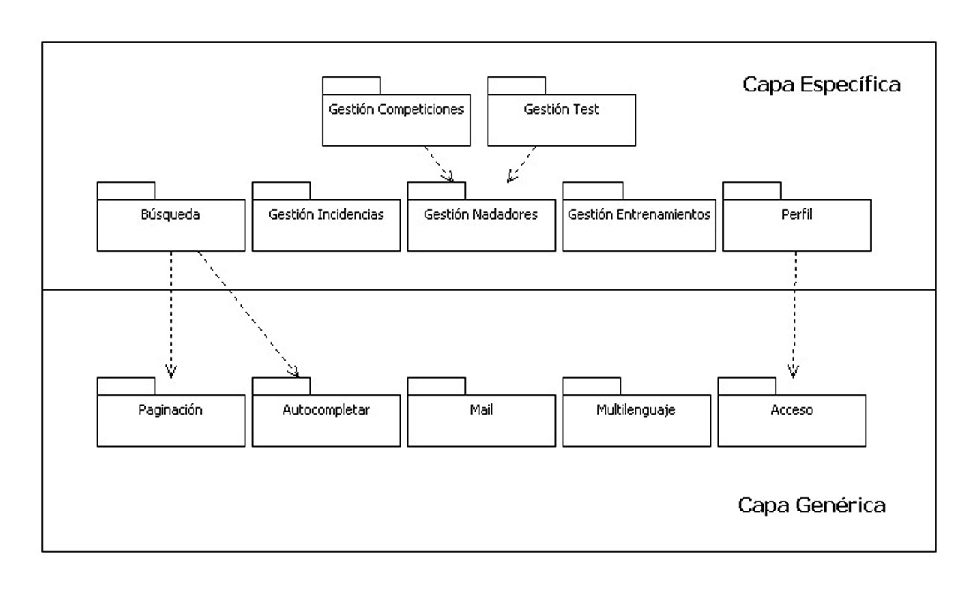
\includegraphics[width=14cm]{./eps/an_diagpaquetes/an_diagpaquetes.eps}
		  \caption{Diagrama de paquetes para el análisis}
		  \label{fig:an_diagpaquetes}
		\end{figure}
		
		En la figura \ref{fig:an_diagpaquetes} se muestran los principales paquetes que se detectan en la aplicación para las capas genérica y específica. Siguen la misma estructura de descomposición del modelo de casos de uso, donde cada uno de los paquetes da soporte a un proceso del negocio.
	% section diagrama_de_paquetes (end)

% chapter analisis (end)